%% V0.1
%% 2020/10/09
%% by Markus Götz, Björn Hagemeier, James Kahn

\documentclass[aspectratio=1610]{beamer}

\usepackage{helmholtzai}

\newcommand\crule[3][black]{\textcolor{#1}{\rule{#2}{#3}}}

\title{Title}
\subtitle{Subtitle}
\author{Firstname Lastname}
\date{YYYY-MM-DD}
\institute{Center}

\begin{document}

\maketitle

\begin{frame}
    \frametitle{Usage}
    
    \begin{enumerate}
        \item Download all files from Github\\~
        \item Edit \texttt{slides.tex} with your favorite editor\\~
        \item Compile the slides by either:\\~
        \begin{enumerate}
            \item Typing \texttt{make} in the directory of \texttt{slides.tex} or\\~
            \item Using a \LaTeX IDE like TeXstudio\\~
        \end{enumerate}
        \item \emph{Note:} make sure to use LuaLaTeX or XeLaTeX as compiler (default in \texttt{make})
    \end{enumerate}
\end{frame}

\begin{frame}
    \frametitle{Slide title}
    \framesubtitle{\textbf{Subtitle} and \emph{more}}
    
    \begin{itemize}
        \item Suppose $a$
        \item Also note b
        \begin{itemize}
            \item This entails
            \item Remember also
            \begin{itemize}
                \item I almost forgot
                \item Envision
            \end{itemize}
        \end{itemize}
    \end{itemize}
\end{frame}


\begin{frame}
\frametitle{Equations}

    \begin{equation*}
        f(x) = \sum_i wx_i^2 + \frac{\beta}{2}
    \end{equation*}
\end{frame}


\begin{frame}
    \frametitle{Columns and Figures}

    \begin{columns}
        \begin{column}{0.4\textwidth}
            \begin{enumerate}
                \item Consider A
                \item ... do not forget B
            \end{enumerate}
        \end{column}
        \begin{column}{0.4\textwidth}
            \centering
            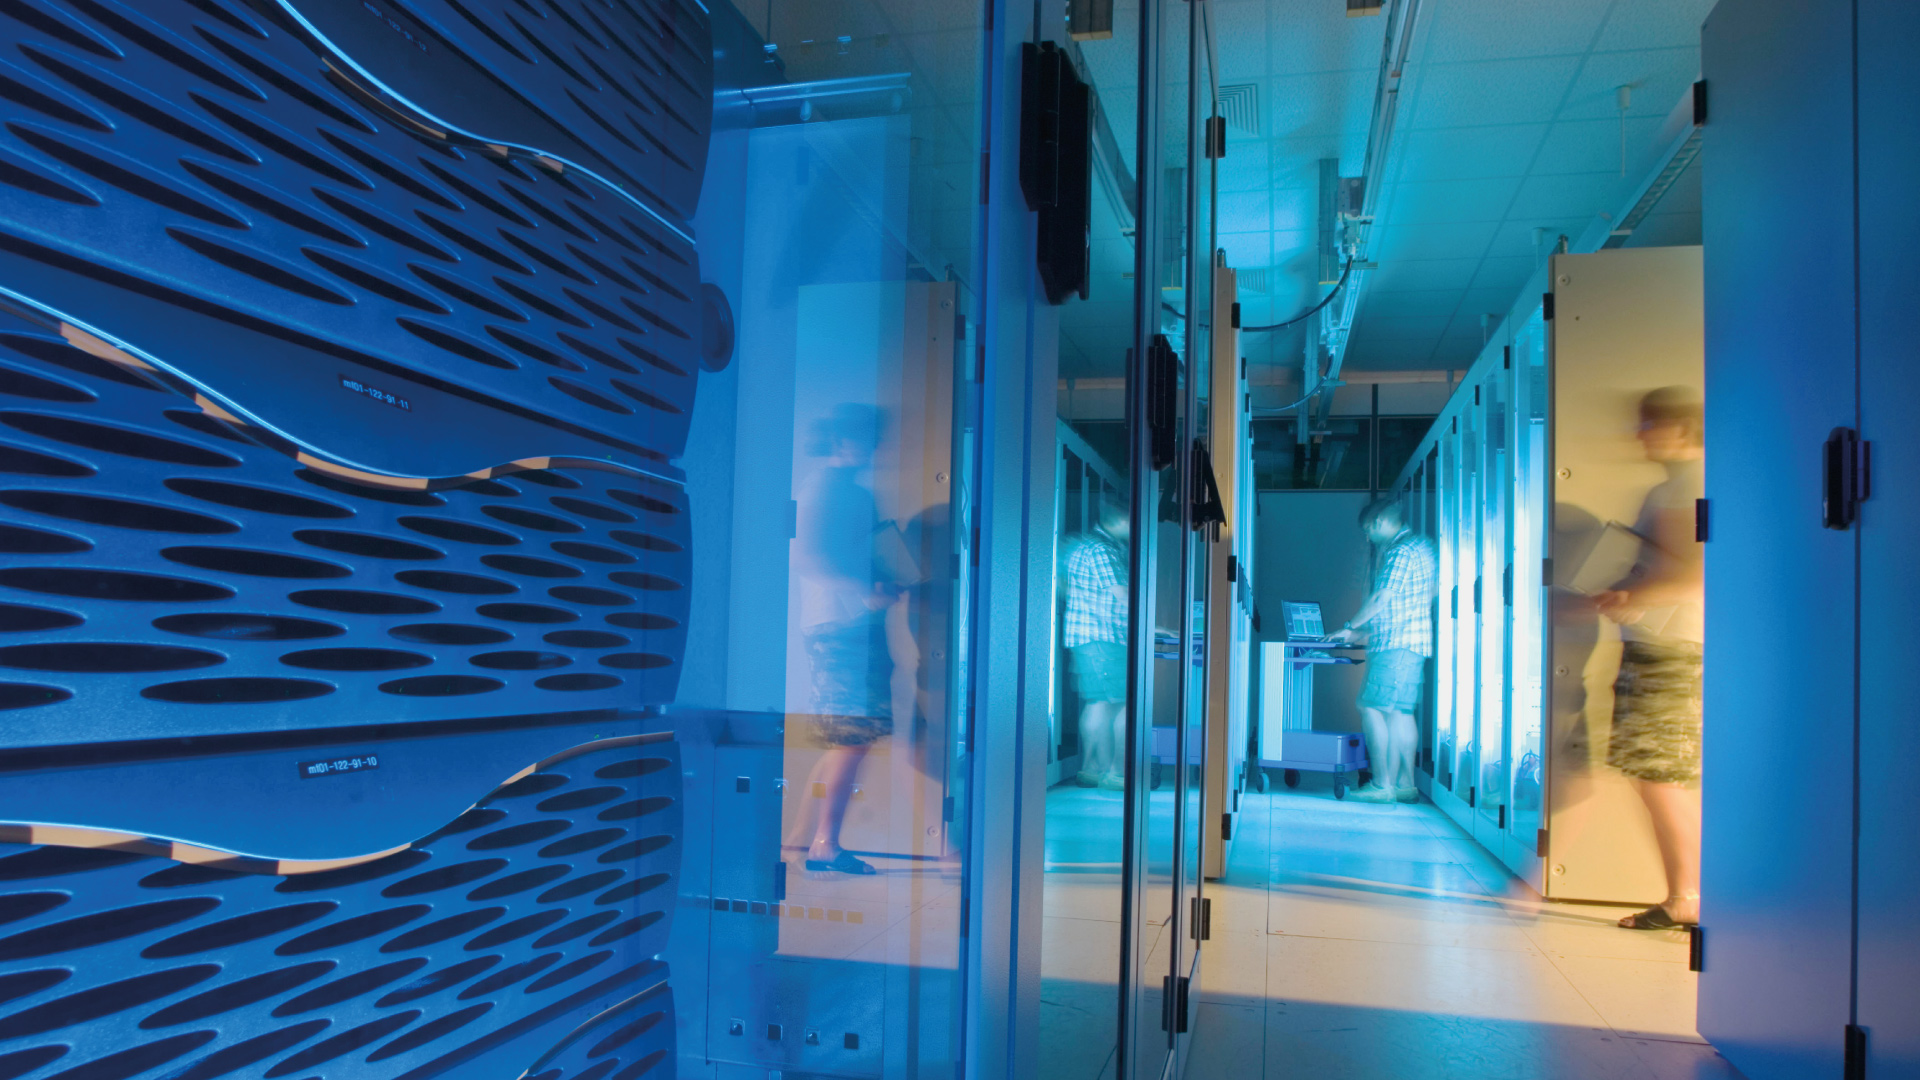
\includegraphics[width=\textwidth]{logos/hgf_key_technologies.jpg}
        \end{column}
    \end{columns}
\end{frame}

\begin{frame}[fragile]
    \frametitle{Code}
    
    \emph{Note the [fragile] specifier next to frame and the code indentation.}
    
\begin{lstlisting}[language=Python]
import numpy as np

def foo(a, b):
    """
    asd
    """
    return a + b + 1
\end{lstlisting}
\end{frame}


\begin{frame}
    \frametitle{Colors}
    \framesubtitle{Basic Definitions}
    
    \emph{The beamer template contains definitions for all Helmholtz colors.}\\
    
    \begin{table}
        \centering
        \small
        \begin{tabular}{cl}
            \textbf{Color} & \textbf{Name}\\\toprule
            \crule[hgfblue]{10pt}{10pt} & hgfblue \\
            \crule[hgfdarkblue]{10pt}{10pt} & hgfdarkblue \\
            \crule[hgfgreen]{10pt}{10pt} & hgfgreen \\
            \crule[hgfgray]{10pt}{10pt} & hgfgray \\
            \crule[hgfaerospace]{10pt}{10pt} & hgfaerospace (short: hgfast) \\
            \crule[hgfearthandenvironment]{10pt}{10pt} & hgfearthandenvironment (short: hgfee) \\
            \crule[hgfenergy]{10pt}{10pt} & hgfenergy \\
            \crule[hgfhealth]{10pt}{10pt} & hgfhealth \\
            \crule[hgfkeytechnologies]{10pt}{10pt} & hgfkeytechnologies (short: hgfkt, hgfinformation) \\
            \crule[hgfmatter]{10pt}{10pt} & hgfmatter \\\bottomrule
        \end{tabular}
    \end{table}
\end{frame}


\begin{frame}
    \frametitle{Colors}
    \framesubtitle{Shades}
    
    \emph{For each color there exist 10 lighter shades, exemplary for hgfblue}\\
    
    \begin{table}
        \centering
        \small
        \begin{tabular}{cl}
            \textbf{Color} & \textbf{Name}\\\toprule
            \crule[hgfblue10]{10pt}{10pt} & hgfblue10 \\
            \crule[hgfblue20]{10pt}{10pt} & hgfblue20 \\
            \crule[hgfblue30]{10pt}{10pt} & hgfblue30 \\
            \crule[hgfblue40]{10pt}{10pt} & hgfblue40 \\
            \crule[hgfblue50]{10pt}{10pt} & hgfblue50 \\
            \crule[hgfblue60]{10pt}{10pt} & hgfblue60 \\
            \crule[hgfblue70]{10pt}{10pt} & hgfblue70 \\
            \crule[hgfblue80]{10pt}{10pt} & hgfblue80 \\
            \crule[hgfblue90]{10pt}{10pt} & hgfblue90 \\
            \crule[hgfblue]{10pt}{10pt} & hgfblue \\\bottomrule
        \end{tabular}
    \end{table}
\end{frame}

\section{Sections look like this}

\end{document}
